% !TEX root = ../journaltemplate.tex

\begin{figure}[h!]
    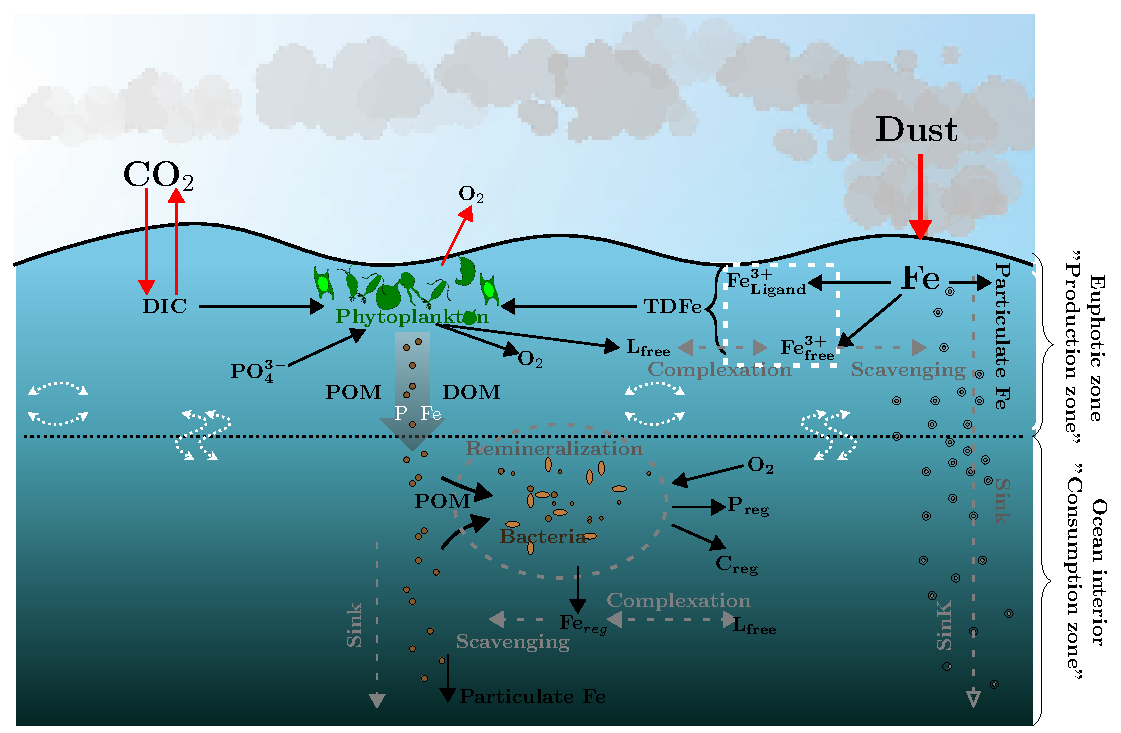
\includegraphics[scale=0.8]{../Paper_Draft/tikz/Fe.pdf}
    \caption{The iron (Fe) cycle in cGENIE. The only source of Fe to the ocean is dust. A fraction of supplied Fe will be complexed with organic ligands (Fe$^{3+}_{ligand}$), kept in free state (Fe$^{3+}_{free}$), and scavenged into particulate organic carbon (POC, Particulate Fe) to sink through the water column. The total dissolved Fe pool (TDFe) will be used by biology to generate particulate (POM) and dissolved (DOM) organic matter. The remineralization process will regenerate nutrients and carbon.}
\end{figure}

\subsection{General model description}

We use a version of the Grid-ENabled Integrated Earth (GENIE) model focused on the carbon (C) cycle, cGENIE muffin v0.9, with three modules: (1) the 3D frictional-geostrophic ocean module, with 16 depth levels and a 36x36 equal-area horizontal grid (constant 10° in longitude and uniform in the sine of latitude), (2) marine biogeochemistry module BIOGEM (Ridgwell et al., 2007), and (3) an atmospheric component of the 2D energy-moisture balance model with prescribed climatological wind fields (Cao et al., 2009). The continental distribution and bathymetry are published in Ridgwell et al. (2007).

For this study, we focused on the biological pump of soft tissues. For this purpose, a co-limitation scheme of iron (Fe) and phosphorus (P) to the C cycle was implemented following Tagliabue et al. (2016). Additionally, a simplified scheme of organic complexing, nutrient removal, and particulate organic C (POC) sink was implemented following the methodology proposed by Parekh et al. (2004, 2006). Table S1 in the Supporting Information summarizes the data sets and values used. The circulation model uses both parameterized temperature (van de Velde et al., 2021), salinity and 33 biogeochemical tracers to describe the interactions between nutrients. In order to make a correct C inventory, tracers and pre-formed nutrients were used following the base configuration of Cao et al. (2009).

In BIOGEM, C sequestration is controlled by biological export. The biogenic uptake of dissolved nutrients, tracers and inorganic C occurs in the ocean euphotic zone (upper 81 m). Remineralization by ocean bacteria (at a 590-m depth) results in dissolution (i.e., regeneration) of inorganic nutrients and C. Finally, the efficiency of the biological pump (P*) is defined in terms of the ratio of the regenerated (Preg) to total (Ptotal) P concentration: $P^{*} = P_{reg}/P_{total}$

\subsection{Model nutrient limitation scheme}

Both P and Fe have low ocean concentrations in many ocean basins, and in order to reproduce their limiting effects on primary productivity we use a colimitation scheme. The co-dependency between the concentration of dissolved phosphate ([PO$_4^{3-}$]) and the biological uptake of C at the surface ocean is expressed as:

\begin{linenomath*}
\begin{equation}
    P:C=1:\left(\frac{[PO_4^{3-}]}{144.9 \mu mol L^{-1}} + 0.006\right)^{-1}
\end{equation}
\end{linenomath*}

n cGENIE, the surface ocean is highly oxygenated and thus most of the Fe input is rapidly oxidized to Fe$^{3+}$ (Figure 2). Iron dissolution is a determining factor in photosynthesis and it will depend on water temperature, salinity, and pH. Total dissolved Fe (TDFe) will be composed of (1) free Fe (Fe$^{3+}_{free}$) and (2) ligand-bound Fe (Fe$^{3+}_{ligand}$). TDFe in the ocean is mostly present as  (~99\%), while Fe$^{3+}_{free}$ is the only species that is susceptible to be scavenged by POC and eliminated from the system when TDFe  is higher than the total concentration of ligands (L$_T$). In turn, L$_T$ consists of a free ligand component (L$_{free}$) and that associated to Fe (Fe$^{3+}_{ligand}$), and is invariant and uniform in the water column (0.1 nM) following Parekh et al. (2005) and Doney et al. (2006).

Finally, the Fe:C ratio is variable and parameterized to depend on TDFe, so that Fe requirements at the cellular level depend on Fe availability. Thus, under higher limitation, less Fe will be required and vice versa (a minimum ratio of 250,000 is imposed during maximum Fe limitation): 

\begin{linenomath*}
    \begin{equation}
Fe:c=\frac{1}{min(250,000,103,700 TDFe-0.4225)}
    \end{equation}
\end{linenomath*}

\subsection{Experimental design}

Six pairs of Holocene-Last Glacial Maximum (LGM) dust deposition rate fields were used as sources of soluble Fe to force cGENIE (for details see Lambert et al., 2021). One of these pairs (Lambert) is derived from paleo-dust observations compiled by Lambert et al. (2015), while the rest are derived from CMIP5 model simulations: Albani (Albani et al., 2014), Takemura (Takemura et al., 2009), Ohgaito (Ohgaito et al., 2018), MIROC-ESM (Sueyoshi et al., 2013) and MRI-CGCM3 (Yukimoto et al., 2012). 

Since the solubility of iron in dust is not well known, a sensitivity analysis was carried out by creating different dust iron solubility fields for each dust deposition rate field. To achieve this, we start by deriving a field of fractional Fe solubility ($\Upsilon_{Fesol}$, \%) in dust based on each of the twelve dust deposition rate fields described in the previous paragraph (i.e., six for the Holocene and six for the LGM), calculated as: 

\begin{linenomath*}
    \begin{equation}
\Upsilon_{Fesol}= \gamma_{Fesol}C_{dust}^{-0.5}
    \end{equation}
\end{linenomath*}

where $\gamma_{Fesol}$ is a scaling factor and $C_{dust}$ is the concentration of dust in the surface ocean layer (see Text S1 of the Supplementary Information for further details). This relationship reflects observations that iron solubility of dust aerosols in weak acid solutions is inversely proportional to atmospheric dust load (Baker and Jickells, 2006).

Additionally, based on these twelve derived iron solubility reconstructions we created new fields by scaling all grid values by the same factor, as well as by scaling values of grid cells located within one of the five High-Nutrient, Low Chlorophyll (HNLC) ocean basins with respect to all other grid cells outside of any given HNLC ocean. In all cases the scaling factors used were 0.33, 0.67, 1.00 (i.e., no scaling factor applied), 2.00, and 3.00. Consequently, the model was forced with a total of 150 Holocene-LGM pairs of dust ($\Upsilon_{Fesol}$) fields. As we are interested in performing a sensitivity analysis of aeolian iron inputs to ocean CO$_2$ drawdown, all additional supplies of Fe associated with sedimentary processes in the ocean were not considered.

\subsection{Simulation}

\begin{figure}[h!]
    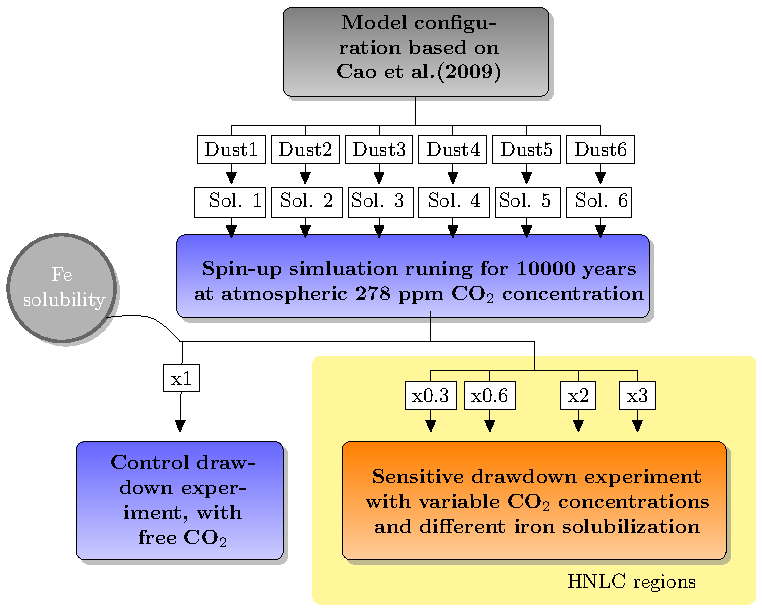
\includegraphics[scale=1]{../Paper_Draft/tikz/Figure3_diagram.tex.preview.pdf}
    \caption{Flow chart describing the experiment design. The gray box shows the general configuration used for spin-up and sensitivity experiment simulations. White boxes labeled Dust 1-6 represent the six Last Glacial Maximum (LGM) and six Holocene dust deposition flux fields used as input to the simulations, while the associated input fields of dust fractional iron (Fe) solubility are represented by white boxes labeled Sol. 1-6. The top blue box represents the spin-up simulations run for each input field of dust flux, using a fixed value for atmospheric carbon dioxide (CO$_2$) concentration. The bottom blue box represents the control simulations run with unprescribed CO2 for each input dust field (six for LGM and six for the Holocene). The bottom yellow box represents the main set of sensitivity experiment simulations, in which for all 12 input fields of dust fractional iron solubility, all grids of a given high-nutrient, low-chlorophyll (HNLC) ocean basin  are multiplied by the same scalar factor. }
\end{figure}

We spun up cGENIE by performing six different 10,000-year pre-industrial experiments in which atmospheric carbon dioxide (CO2) concentration was fixed at 278 ppmv (Figure 3). Each of these six simulations was forced by a Holocene dust ($\Upsilon_{Fesol}$) field. Starting from the end of each spin-up, we ran global and regional sensitivity experiments as described in the previous section for the Holocene and LGM, allowing the model to run for an extra 10,000 years. Finally, we took the mean of the last 500 years of CO2 concentration and carbon export rate from each simulation.
